%%%%
%% Load the class. Put any options that you want here (see the documentation
%% for the list of options). The following are samples for each type of
%% thesis:
%%
%% Note: you can also specify any of the following options:
%%  logo: put a University of Edinburgh logo onto the title page
%%  frontabs: put the abstract onto the title page
%%  deptreport: produce a title page that fits into a Computer Science
%%      departmental cover [not sure if this actually works]
%%  singlespacing, fullspacing, doublespacing: choose line spacing
%%  oneside, twoside: specify a one-sided or two-sided thesis
%%  10pt, 11pt, 12pt: choose a font size
%%  centrechapter, leftchapter, rightchapter: alignment of chapter headings
%%  sansheadings, normalheadings: headings and captions in sans-serif
%%      (default) or in the same font as the rest of the thesis
%%  [no]listsintoc: put list of figures/tables in table of contents (default:
%%      not)
%%  romanprepages, plainprepages: number the preliminary pages with Roman
%%      numerals (default) or consecutively with the rest of the thesis
%%  parskip: don't indent paragraphs, put a blank line between instead
%%  abbrevs: define a list of useful abbreviations (see documentation)
%%  draft: produce a single-spaced, double-sided thesis with narrow margins

\documentclass[msc,cs,logo,abbrevs,11pt]{infthesis}

\usepackage{natbib}
\usepackage{hyperref}
\usepackage{url}
\usepackage{listings}
\usepackage{graphicx}
\usepackage[normalem]{ulem}
\usepackage[skins]{tcolorbox}
\usepackage{xspace}\usepackage[inline]{enumitem}

\newcommand{\dpy}{dispel4py\xspace}
\newcommand{\Dpy}{Dispel4py\xspace}

\newcommand{\THE}[1]{the #1}

\newcommand{\tesieve}{sieve of Eratosthenes\xspace}
\newcommand{\teSieve}{Sieve of Eratosthenes\xspace}
\newcommand{\ttesieve}{\THE{\tesieve}}
\newcommand{\tsieve}{\tesieve}
\newcommand{\tSieve}{\teSieve}
\newcommand{\ttsieve}{\THE{\tsieve}}
\newcommand{\ttSieve}{\THE{\tSieve}}

\title{Making \dpy dynamic}
\author{Rui Zhao s1623641}

%% If the year of submission is not the current year, uncomment this line and 
%% specify it here:
% \submityear{1785}

%% Optionally, specify the graduation month and year:
% \graduationdate{February 1786}

%% Specify the abstract here.
\abstract{%
\sout{This is the abstract containing the main content of the dissertation document. Abstract is with title page.}
}

\begin{document}
\begin{preliminary}
\maketitle

\begin{acknowledgements}
Many thanks to my mummy for the numerous packed lunches; and of course to
Igor, my faithful lab assistant.
\end{acknowledgements}

\standarddeclaration

%% Finally, a dedication (this is optional -- uncomment the following line if
%% you want one).
% \dedication{To my mummy.}

\tableofcontents

%% If you want a list of figures or tables, uncomment the appropriate line(s)
% \listoffigures
% \listoftables

\end{preliminary}

%%%%%%%%
\chapter{Introduction}
We report the exploration of improvements to a workflow management system that enables scientific methods to be encoded using data streaming. We report and evaluate a prototyping dynamic mapping of processes onto computational platforms.

The prevalence of workflow systems as a means of ongoing computational and data driven methods motivates this work. The nature of these systems and their data-streaming variants are introduced to set the context for the experiments. We then introduce \dpy as well as possible enhancements to it, and briefly describe our design to tackle them.

Science and researchers have gone through many eras and stages, and are facing a new paradigm today -- data-intensive science \cite{hey2009fourth}. Many current research campaigns involve producing large quantities of data and analysing them. As always, researchers need to develop methods themselves and then perform computation and analyse the results. Consequently researchers need flexible tools to help organise, implement and perform their methods. Here is how workflows and workflow management systems join the story: researchers can describe their methods by means of workflows and execute them in a workflow management system.

The scientific workflow (``workflow'' for short) is a technique used to organize and manage scientific computational jobs. By using scientific workflows, each computational job is decomposed into several (sub-)tasks which are connected by their dataflows (data dependencies). Hence, every workflow can be easily re-designed to suit specific needs by modifying its (sub-)tasks. Moreover, each (sub-)task can be seen as a module which can be developed independently, and they can be reused in different workflows so researchers can easily design new workflows by selecting and combining different modules.

The software system / framework used to execute scientific workflows is called a workflow management system (WMS). Researchers only need to provide the workflow and relevant input data, then the rest of the story will be automated by the WMS. Usually WMSs will parse the given workflow and map / assign tasks to some kinds of distributed computation platforms, such as clusters.

\Dpy is a data-streaming workflow management system written in Python \cite{doi:10.1177/1094342016649766}. It does not introduce new execution platforms, but maps the workflow into some existing platforms such as MPI \cite{MPI_forum} or Apache Storm \cite{apache_storm}. As Python is widely available, the computers / servers on which the execution will happen don't need extra configurations. That said, as long as the libraries that tasks / PEs used are installed, \dpy can take control of the whole executing process and use the platform existing with no require of users' attention. If the tasks / PEs are written completely in Python, then no configuration is needed at all.

Currently, as far as we know, the workflow going to execute should be constructed solidly before its execution and is not subjected to change during its execution in most WMSs (which is all of the \emph{data-streaming} WMSs and most of the \emph{task-oriented} WMSs \footnote{The differenc between \emph{data-streaming} WMSs and \emph{task-oriented} WMSs will be detailed in the ``Background'' chapter.} with only a few exceptions, such as DAGMan for Condor \cite{couvares2007workflow}) and the deployment (\ie which node will execute which sub-task) happens at the beginning of the execution, which means the workflow as well as its deployment will be static during the execution. However, some computations can be represented more naturally in a dynamic way and some nodes (especially the ones near the end of the workflow) will actually be waiting for a long time before data coming in. As a consequence, it may save time or resources not to deploy all nodes in the beginning and may save nodes (therefore lower computational resources needed) if we can collect and re-allocate nodes that have finished producing outputs. To tackle this weakness, we extended \dpy to give it the ability to dynamically / incrementally deploy (sub-)tasks to computer nodes and a new semantics, \emph{dynamic expansion}, to workflows. In the meantime, our new system keeps backward compatibility so that existing workflows can still be correctly executed.

The ability to deploy (sub-)tasks to computer nodes only when needed is called \emph{incremental deployment} by us. We introduce a coordinator node that knows the global structure of the workflow and is in charge of node deployment, and degrade the rest of the nodes to executors / workers that only know themselves and their neighbours (\ie the nodes its input and output connections are connected with). Every time an executor needs new output targets, it requests that node and gets response from the coordinator. After all executors have finished their work (\ie no more inputs and outputs), they will all be shut down by the coordinator (and the coordinator also shuts itself down), so the whole execution is then finished. We use carefully designed signals / communications (which will be detailed in the \rcpt{Incremental Deployment} chapter) to ensure the execution and shut-down process's correct execution. This master-slave-like structure acts as a demonstration of possibilities for \dpy or other similar systems and is subject to change (\eg multiple coordinators \footnote{More details are presented in the \rcpt{Future Work} chapter.}) for future development.

The new semantics to grow the workflow dynamically according to certain rules is called \emph{dynamic expansion}. In order to keep backward compatibility, we add a special mark (implemented as a \lstinline|property| with default value) to the Processing Element (PE) indicating whether or not the task can be further expanded. In order to encode the expansion rules, we add special connections (called \emph{circuit connection}) and corresponding methods to define them. The details will be described in the ``Dynamic Expansion'' chapter.

Introducing these two new extensions enables us (or other researchers / developers) to make further optimisation and extensions. For example, in the original \dpy system, we can only collect performance data of past runs and use them to direct the deployment of future runs; but now, we can also collect the performance data during the incremental deployment (\ie on-the-fly) and use these data to aid the following deployment of the same execution.

The remaining part of this document will be organised as follows: first, we will present some terminology which may lead to confusion if not stated clearly; following that, we will present necessary background information; then we will detail the extensions we have done in separate chapters; after that, we will present the measurement and evaluation for them; finally, we will draw a conclusion.

	
\chapter{Terminology}
To avoid confusion, we present how we use terminology in this document.

\newenvironment{term_box}{\begin{tcolorbox}[enhanced,width=5in,size=fbox,
    fontupper=\large\bfseries,drop shadow southwest,sharp corners]}{
\end{tcolorbox}}

\begin{itemize}

\item \emph{PE} is short for Processing Element, which is the basic component of dispel4py graph (detailed later). In most cases, a \emph{PE} is equivalent to a \emph{task} in a workflow. We will use the term \emph{PE} instead of \emph{task} when talking about dispel4py.

\item \emph{Task} means a specific computation job in a workflow. Each workflow consists of many \emph{tasks}. Sometimes, we use \emph{(sub-)task} instead of \emph{task} for clarity, but they mean the same. It will be used when we are not talking specifically about dispel4py.

\begin{term_box}
Although \emph{PE} and \emph{task} are usually interchangeable in our context, there is a difference in the common case. Normally, \emph{task} is used in the task-oriented environment so they will exit after processing; \emph{PE} is a term in dispel4py (which is a \emph{data-streaming} system), so they will keep running and waiting for more data after processing a unit of data until no more data coming in.
\end{term_box}	
	
\item \emph{Node} means a computer in a network, usually one executing some computational jobs. Because modern computers usually consists of many \emph{core}s, it is not ideal to consider each of the computers (which may have different number of \emph{cores}) as a standalone entity. A better practice would be considering each \emph{node} as a single-core machine.

\item \emph{Core} refers to a CPU core. A modern computer consists of many \emph{core}s, so \emph{core} is not the same as \emph{node}. Usually we won't use \emph{core} directly because programming doesn't directly operate on \emph{core}s.

\begin{term_box}
Although \emph{node} and \emph{core} are different in definition, we would usually consider each \emph{node} as a single-\emph{core} machine, which means they are the same in our context (and we prefer to use \emph{node}).
\end{term_box}	

\begin{term_box}
Notice that each \emph{task} or \emph{PE} is usually programmed with no aware of multi-cores. However, they can wield multi-threading to perform necessary light-weight (i.e. not computational-intensive) tasks (such as communication).
\end{term_box}
	
\item \emph{Unit} means a piece of data produced by some \emph{task}s / \emph{PE}s. Usually, each \emph{task} / \emph{PE} will consume or produce many \emph{unit}s of data with the same format (on each data stream).

\item \emph{Data-streaming} means the data produced is not going to be cached on disk (or other permanent storage devices), but to be directly sent (\ie streamed) to the corresponding receiver node(s).

\item \emph{Pipeline} refers to the property that the following nodes start to process data when the first \emph{unit} of data is supplied (\ie it does not wait until all data has been produced by upstream \emph{PE}s).

\end{itemize}



\chapter{Background}
Because scientific workflows decompose computational jobs into smaller (loose-coupling) pieces, tasks, and use dataflow to connect them, various strategies can be chosen to accomplish the execution (and management) of workflows. Different choices of strategies lead to different behaviours of the workflow management systems (WMSs) and make them suitable for different scenarios. In this chapter, we introduce the growing use of scientific workflows, providing three examples in different disciplines, present the classification of workflow management systems (WMSs) and introduce some basic concepts of the WMS on which our work is based, \dpy. During the journey, we also gradually show why we favour data-streaming WMSs and why we choose \dpy.

\section{Workflow on Nowadays}
The grow and expansion of scientifc workflows went through many years. During the past 10 years, workflows have been adopted by growing number of communities and have influenced almost all researchers \cite{ATKINSON2017216}.
% Because of the abstract definition of workflows, researchers can always produce new methods and tools to refresh current implementations or methods. Malcolm \etal \cite{ATKINSON2017216} presented four benefits of it:
%\begin{enumerate}
%	\item The encoded meaning can sustain during the evolvement of technologies because they are largely independent of implementation.
%	\item The platforms can be mapped to are unlimited as of the semantics.
%	\item Components are easily reusable and re-designable.
%	\item Inter-discipline sharing is easy.
%\end{enumerate}

Many diciplines use workflows to perform their computational jobs. For example, in a recent paper about a new framework for gravitational wave detection \cite{gwave}, \citeauthor{gwave} use the workflows provided by PyCBC \footnote{https://ligo-cbc.github.io/} to perform the actual gravitational wave detection job. In seismology, seismic ambient noise cross-correlation, which is an important job for preprocessing / denoising raw data gathered, is often encoded as workflows and executed by a WMS (e.g. a hybrid system, Asterism \cite{Asterism}, uses seismic ambient noise cross-correlation as their demonstration). A recent workflow management system called DALiuGE \cite{wu2017daliuge} is demonstrated, in production, capable to process vary large quantities of data and is going to be used, as a prototype, in a consortium of Square Kilometre Array (SKA).

Although great progress and plenty of successful work (including those described above, and others \eg \cite{berriman2007generating} \cite{berriman2010application} in astrophysics, \cite{aiche2015workflows} in biochemistry) have been made, many areas are still under exploration in the field of workflow-related tools. For example, in the past time, most WMSs adopt the task-oriented style which may touch the bottleneck with the growing volume of scientific data whereas data-streaming style WMSs can significantly solve this problem \cite{doi:10.1177/1094342016649766}. Although we have the disk storage space, as Kryder’s law \citep{Kryders_law} pointed the storage density can double every 14 months, the IO speed doesn't increase that fast so caching the data of every stage onto disk will eventually become a huge bottleneck for task-oriented WMSs, unless new storage technologies emerge.

Another field is the workflow-sharing technologies. Different systems have different techniques to set up workflows or tasks, which may involve programming languages and paradigms. Therefore, although systems like myExperiment \cite{de2008design} and CrowdLabs \cite{Mates2011} exist, it is still hard to share tasks and workflows in a domain or implementation independent way. The only work we are aware of is the work by \citeauthor{GARIJO2017271} \cite{GARIJO2017271} which describes the semantics and a system to share workflows and tasks in the sense of the actual task they describe. 

\section{Task-oriented and Data-streaming}
Because the term workflow doesn't describe any details or standards, different systems usually use different methods to construct, manage and execute workflows. These systems are called workflow management systems (WMSs). Because each of them is composed of different trade-offs in their design, different WMSs have different characteristics and can not be roughly unified.

We see the way how WMSs schedule tasks and transport data as their main difference. Therefore we divide WMSs into these two types:
\begin{enumerate}
	\item Task oriented
	\item Data streaming
\end{enumerate}

\textbf{Task-oriented} WMSs usually decompose the workflow into each task, and execute them separately in different phases / stages. The data produced by each task will usually be stored to disk and feed into the following task (and then may be deleted). Systems like Kepler \cite{ludascher2006scientific}, KNIME \cite{Berthold:2009:KKI:1656274.1656280}, Galaxy \cite{blankenberg2010galaxy} and Pegasus \cite{deelman2015pegasus} are all developed as task-oriented workflow management systems and they are the majority of WMSs. The benefit of task-oriented WMSs is they have the entire control of the workflow's execution and can schedule the deployment according to needs (\ie the user can easily stop the execution at some point); they can also provide better fault-tolerance because data of each stage are cached on disk. However, this property is also its weakness: splitting tasks into stages will force a latter task to wait until all its previous tasks has finished, so the time needed will be longer. Moreover, it won't be able to support a continuous infinite data source because the stage used to execute that source will be infinite.

\textbf{Data-streaming} WMSs, on the other hand, stream small units of data directly from the prior tasks to the following tasks, often in a pipeline fashion. It is significantly different to task-oriented WMSs which move entire data between stages, and each unit of data can be arbitrarily complex (or arbitrarily simple such as a filename) in data-streaming systems \cite{doi:10.1177/1094342016649766}. Therefore, it will naturally support infinite data sources and there is no stages so no time will be wasted in waiting for the entire dataset is produced. As a result, the total execution time will be lower and users can get preliminary (partial) data when the first unit of outputs come out of the last task(s). On the contrary, fault tolerance of data-streaming WMSs will be weaker because there is no default mechanism caching intermediate data (so if a node fails, the whole workflow will need to restart). Even though, this weakness can be alleviated a bit by introducing intermediate tasks which passes the data while persisting them.

Although there are already several systems in the field, they don't completely satisfy the needs of current or near-future researchers \cite{•}. For example, with the development of IoT devices \cite{•}, there is a growing number of continuous infinite streams, \eg generated from sensors, which can be make use of. We can imagine researchers using continuous infinite streams as sources in workflows to make, for example, preliminary transformations to raw data in the future. However, because many systems are task-oriented, they are locked down to finite data so are not able to support this fashion. Therefore, we can say that data-streaming is the future. Thus, we expect to give mor e dynamics to data-streaming WMSs to better satisfy not only today's but also tomorrow's needs of researchers.

\section{Dispel4py}
\Dpy is a data-streaming pipeline-fashion WMS. It it built on top of the design of the Dispel workflow specification language \cite{atkinson2012data} while aligns more to scientists \cite{doi:10.1177/1094342016649766}. The most significant benefit of \dpy is that it maps the execution of workflows automatically to other platforms (\eg MPI) so it requires no user attention as long as the libraries needed are properly installed. This characteristic makes \dpy a comprehensive system, which is lacked by many systems. Moreover, because of the wide availability of Python, the large number of high-quality libraries for Python, it is easy to write new workflows or PEs (see next paragraph) for \dpy, and the ability to interoperate with C/C++ codes makes it possible to wrap existing workflows to execute in \dpy. These make it very easy to migrate to or use \dpy, and  PEs written in pure Python are usually platform-independent so sharing PEs and workflows is also very easy in \dpy.

In \dpy, the basic component is called Processing Element (PE). Generally, each PE corresponds to a task in the workflow. Each PE has zero or more inputs, and zero or more outputs (but not likely to be both zero because it's useless). A PE itself doesn't know where its inputs are from and where its outputs are to, which decouples PEs.

A workflow in \dpy is constructed by connecting output connections from one PE and input connections from another PE.

An example (split-merge) of workflow construction is made in \dpy is shown in Listing \ref{lst:wf_example} (taken from the original \dpy paper \cite{doi:10.1177/1094342016649766}).

\begin{lstlisting}[frame=single,caption={Example code of workflow construction in \dpy},captionpos=b,label={lst:wf_example},language=Python]
from dispel4py.workflow_graph import WorkflowGraph

pe1 = WordNumber()
pe2 = CountWord()
pe3 = Average()
pe4 = Reduce()

graph = WorkflowGraph()
graph.connect(pe1, 'output1', pe2, 'input')
graph.connect(pe1, 'output2', pe3, 'input')
graph.connect(pe2, 'output', pe4, 'input1')
graph.connect(pe3, 'output', pe4, 'input2')
\end{lstlisting}

\defTerm{PETmpl}{PE template}
\defTerm{PEInst}{PE}
\defTerm{PEDup}{PE instance}

There is a conceptual difference between \tPETmpl{}s, \tPEInst{}s and \tPEDup{}s, which may worth mentioning: a \tPETmpl is the logic (template) for processing data, usually implemented as a Python class; a \tPEInst is an instance (after construction) of such a class (\tPETmpl); \tPEDup is used only when we are talking about the (deliberate) duplications (copies) of the same \tPEInst. A \tPETmpl can be used to construct many different \tPEInst{}s and they can all behave differently because of, for example, the different parameters used to call the constructor. By default, each \tPEInst only has one \tPEDup so we usually don't distinguish between them (and we will favour the term \tPEInst); however, when deliberate duplication happens (\eg for better throughput as suggested by \citeauthor{doi:10.1177/1094342016649766} \cite{doi:10.1177/1094342016649766}), we will talk about \tPEDup{}s for better clarity.

The execution of \dpy is done by mapping the workflow to an execution platform (\ie an DCI), such as MPI, Storm or Multiprocessing which are currently supported by \dpy. This mapping behaviour is the benefit of the abstraction that \dpy brings because developers for workflows don't need to know anything about the platform (\eg hardware or middleware) that the workflow is going to be executed. This behaviour also gives the developers of \dpy freedom to optimize or extend the actual working procedures of \dpy without needing to worry about backward compatibilities too much.

For example, one of the current ``problem'' in \dpy is that it maps the whole workflow graph at once in the beginning, which may consume much time. As the method how workflows are constructed presents, the workflow in \dpy is a directed acyclic graph (DAG). Therefore, we can perform topological sorting to the graph, and obtain the sources by picking up the nodes with zero in-degrees. Thus, it is possible that we can deploy nodes only when needed (\eg when there are data sending to it) so we don't have to allocate all the resources in the beginning. This is the basic point of our first modification - \tincdep. By using this way, out modification works a bit similar to task-oriented WMSs which also use topological sorting for this purpose.

But we don't stop here - we also make use of the dynamics that \tincdep provides to achieve other goals. That is: because we can deploy PEs incrementally, we can also perform other modification to out workflow graph incrementally according to some rules. This is how our second target, \tdynexp, is done: to dynamically expand the workflow according to needs.



\chapter{Use Case}
We present here two examples that are used to explore the semantics and performance of \dpy. We require to retain all prior semantic interpretations of workflows but introduce new ones that depend on dynamic determination of the generated graph.

We will introduce them separately in the hope that it is more clear to read.

\section{\tSieve} \label{sec:uc_sieve}
We first present \ttsieve which is a very simple yet useful algorithm. We present its basic idea, the common parallel algorithm for \ttsieve and the difficulty to construct it in the current semantics of \dpy (which is one of the motivations of our work).

The known earliest sieve algorithm is \ttesieve given by an ancient Greek mathematician \cite{o2009genuine}. The basic idea of \ttesieve is that we cross out all multiples (up until a certain upper boundary) of every prime at the time we encounter a new prime.

As we are using prime sieves as demonstration, we mainly focus on the correctness and simplicity rather than the efficiency. Therefore, we can simply change the structure of \ttesieve into a distributed manner: each node is responsible for one prime, and it crosses out all multiples of the prime it is responsible for; a continuous integer producer produces integers to the first sieve; each sieve node sends the un-crossed integers to the next sieve node.

As the description of the distributed sieve shows, we need each node responsible for each prime, which means we need to allocate at least number-of-prime sieves before executing the workflow. However, since we don't yet know which those primes are, we also don't know the number of them. This leads to a chicken-and-egg problem. One possible practice is to estimate the number of primes in the region and allocate that many nodes.

\newcommand{\cdIntGen}{\lstinline|IntegerGenerator|\xspace}
\newcommand{\cdSieve}{\lstinline|PrimeSieve|\xspace}

In the current \dpy system, to construct a workflow for this, we first define two kinds of PEs:
\begin{enumerate*}
	\item \cdIntGen which continuously produces integers from 2 up to a certain limit;
	\item \cdSieve which keeps a prime number it is responsible for and passes all number which is not a multiple of that prime. Then we need to connect the output of \cdIntGen to the input of \cdSieve , and then chain as many \cdSieve{}s as we need.
\end{enumerate*}

To define the graph, we need exactly two numbers: one is the range (\ie the maximum number) and the other is the number of primes in this region. Typically, we need to first find out the number of primes in this range by running a prime generator elsewhere, and then use it to construct the workflow. If we set the number smaller, the workflow can execute, but will produce unreliable numbers when the actual number of primes exceeds the number of sieves defined in the workflow graph; if we set the number larger, the correctness of the workflow execution will then depend on how outputs from the sieves are connected to the successor nodes (e.g. if only the final sieve is connected to the successor nodes, then there will be no outputs from the last sieve and, therefore, no inputs to the successor so it will behave erroneously).

Two problems emerge from this construction method:
\begin{enumerate}
	\item The chicken-and-egg problem previously mentioned;
	\item A different graph is needed when we want to change the maximum number.
\end{enumerate}

Both of them are quite unsatisfying for researchers / developers because they both involve manual inspection apart from the basic workflow (especially task) design. Researchers, \eg us, would prefer a more unified automatic way in which we only need to define once without calculating the number of primes before execution.

This motivates our research and we present the new semantics called \emph{dynamic expansion} (in addition to \emph{incremental deployment}) to support this expectation. In the new semantics, we no longer need to manually assign many sieves. Instead, we only need to define the \cdSieve automatically expandable (by setting the \lstinline|repeatable| property to \lstinline|True|) and describe when to expand it (by connecting \lstinline|circuit|). Moreover, in our new system, another new use case is available: to find certain number of primes - by making the \cdSieve nodes aware of their status and no longer expand more sieves (it will be more efficient if \emph{backward shut-down propagation} is implemented). Details will be described in the Dynamic Expansion chapter.

\section{Seismic cross-correlation}
(TO BE CONSTRUCTED)

	
\newcommand{\defNode}[1]{%
  \expandafter\def\csname nd#1\endcsname{\emph{#1}\xspace}}
\newcommand{\defNodes}[1]{\forcsvlist{\defNode}{#1}}

\chapter{Incremental Deployment}
In this chapter, we present the \tincdep we introduced for further extension or optimisation of \dpy. We first briefly restate why we introduce \tincdep and our expectation of \tincdep. After that, each section of this chapter contains one main aspect of \tincdep, including the expected behaviour of \tincdep, the semantics changes due to \tincdep and how \tincdep works, except for the last two sections -- the second last section presents an example of \tincdep, and the last section presents how we implement \tincdep in \dpy (including what issues we encountered and how we solved them).

We expect, as said in the Background chapter, future researchers would need to design workflows reading data from continuous infinite data streams. In this situation, the execution time of the workflow will also be infinite unless manually shut down. Therefore, it is infeasible to use past performance data from an ``infinite workflow'' to guide the deployment of future runs of the same workflow. A more dynamic on-the-fly way of deploying PEs to nodes is needed to support possible optimisations. This is one of the reasons we introduce \tincdep.

The second reason is that we expect to support a more natural way to design workflows to accomplish tasks such as the \tsieve we discussed in \ref{sec:uc_sieve}. Details of why we need \tincdep to support it will be discussed in the \rcpt{Dynamic Expansion} chapter.

There is also another reason: we want to minimize the initialization cost for the execution of workflows and spawning, connecting and deploying nodes cost resources, especially time. We expect spawning and deployment on-the-fly can save time in some cases.

\section{Deployment Behaviour}
As \tincdep is the new extension we introduced, we shall first describe the expected behaviour of it as well as a brief comparison against the old system.

In the current \dpy system, when \dpy wants to deploy a \tPEInst to nodes, it will first analyse the workflow to extract the topology and then map \tPEInst{}s to nodes and leave them executing without any more management. The number of nodes used in execution should be assigned prior to execution and is not subject to change during the execution.

We want to introduce more dynamic behaviours, so our expected behaviour should be like this:
\begin{enumerate}
	\item The user doesn't need to know the actual number of nodes needed to execute a workflow (however, the user \emph{can} know that).
	\item The \dpy system will deploy and run only the source \tPEInst{}s in the beginning, rather than all \tPEInst{}s at once.
	\item Other \tPEInst{}s will be deployed during running and each \tPEInst should be deployed exactly once so data transmission won't go wrong because of this late-deployment behaviour.
	\item When a unit of data is going to be sent through an output connection, it will go to the correct destination.
	\item If the output connections of more than one \tPEInst{}s are connected to the same input connection of another \tPEInst, the data sent through these output connections will go to (the same input connection of) the same \tPEInst. Similarly, if one output connection is connected to multiple input connections, the same data will be sent to all input connections.
	\item A \tPEInst should shutdown when there is no more data to produce.
	\item If a \tPEInst never receives any data from any input connections, this \tPEInst doesn't need to be deployed.
\end{enumerate}

To satisfy all these needs, especially the 2nd and 5th points, we need a mechanism to synchronize the knowledge of \tPEInst{}s so no duplicated deployment or loss of data will happen. Because of the nature of distributed computing, we couldn't, at least during the time, find a low-cost way (\ie without many signalling rounds) to guarantee these requirements in a fully de-centralized manner. Therefore, we introduced a coordinator to handle the deployment. We will show, in \ref{sec:incdep_coord}, that our communication strategy is the minimal possible.

To put all these together, the deployment behaviour now is:
\begin{enumerate*}
	\item The coordinator will be launched first in the beginning
	\item The coordinator analyses the workflow and deploys the source \tPEInst{}s (\ie \tPEInst{}s without any explicit input connections).
	\item the coordinator deploys the successor \tPEInst to a node when a \tPEInst needs to send data through an output connection which is connected to a input connection of the successor.
\end{enumerate*}

\section{Revised Semantics for Sending Data}
We briefly mentioned when sending data through an output connection, the coordinator is responsible for deploying the successor \tPEInst{}(s). Here we present how the semantics for sending data has changed and how this is reflected in our implementation of sending data.

In the old \dpy system, because all \tPEInst{}s are deployed in the beginning, all nodes are completely aware with which input connection of which node is an output connection connected. As a result, when an output is produced, the node knows naturally where it will go to. However, because \tPEInst{}s are deployed dynamically when we introduce \tincdep, all nodes lose this knowledge so this semantics is subject to change.

In \tincdep, when a \tPEInst produces a unit of data and sends it through an output connection, this action triggers a lookup to find the correct targets (both input connections and nodes). If the targets have not been deployed yet, the send action will hang up to wait for the completion of the deployment (which is performed by the coordinator) of the targets and then the send action proceeds.

In our implementation, when a \tPEInst produces a unit of data, the node (which runs the \tPEInst) will communicate with the coordinator to request the destination(s) of the output connection. Then it waits for the reply from the coordinator to tell it where that data should be sent to. When it receives the reply, it caches the information (reply) and when next time it is going to send data through the same output connection, it will use the cached information instead of communicating with the coordinator a second time. 
The deployment strategy and process is hidden to the execution nodes, so their main job is still executing the \tPEInst.

It is clear that in this strategy we only add an inspection to the procedure for sending data: to acquire the destination from the coordinator the first time an output connection is used. The rest part of the existing procedure remains unchanged.

\section{Target Selection of Deployment}
What happens during the time the execution node waits for the reply from the coordinator? The coordinator finds the successor \tPEInst{}s which have input connections connected to that output connection, and deploys the \tPEInst{}s to some nodes.

The step to find the successor \tPEInst{}s is fairly simple: the input and output connection pairs are seen as edges in a graph and the coordinator did a topological sort in the beginning so it can barely lookup the result.

When the coordinator knows the successor \tPEInst{}s, it will need to deploy them correspondingly to some nodes. In our system, we perform a plain lookup in the table which contains the status (busy or free) of nodes, and use the first enough free nodes. We are aware that there is a potential optimisation for selecting the nodes to deploy the \tPEInst{}s, such as considering the network speed between the nodes, or considering the computational capability of nodes. However, because of the time limit, it is not possible to accomplish it in our MSc project.

During the lookup, if there is no enough nodes available (free), the coordinator will spawn more nodes and try again. We can use different strategies to decide the number of nodes to be spawned, but we only use a constant for now.

\section{The Coordinator} \label{sec:incdep_coord}
The sections above only talked about the general role and some concrete aspects of the coordinator. In this section, we present how the coordinator works when handling its main job.

The coordinator first performs a topological sorting to the workflow graph in the beginning, and stores which output connection (and the \tPEInst) is connected with which input connection in a quick lookup table (\eg a hash table). It then deploys the source nodes which have no input connections (\ie zero in-degree). The coordinator stores a record (array) which keeps the status of every execution nodes, to track whether they are busy (has a \tPEInst deployed deployed at the moment) or free (has no \tPEInst deployed at the moment), and also the \tPEInst each busy node is running.
Then, the coordinator waits for signals (\ie communications) from the execution nodes after sources are deployed.

During waiting, when the coordinator receives a signal which requires the successors of an output connection, it looks up what input connections and \tPEInst{}s are connected with this output connection, and then checks each of the \tPEInst{}s in the record to see if it is already deployed. For each of those undeployed \tPEInst{}s, the coordinator will deploy it to a node and record this deployment. After all these \tPEInst{}s are deployed, the coordinator replies to the requester with the input connections and the nodes where these \tPEInst{}s are deployed.

It is apparent that there is no need for a node to request for the successors of the same output connection more than once because the deployment won't be changed, so each execution node will cache the reply (or any modifications to the reply) locally. It is also apparent that there is no need for the coordinator to send an ``ack'' back to the requester when receiving the request or for the requester to send an ``ack'' back to the coordinator when receiving the reply from the coordinator, because there is no subsequent actions after each of these signals as long as we can guarantee each message will eventually arrive (which is true under MPI).

When deploying the \tPEInst, the coordinator sends the information necessary for a node to construct the \tPEInst. In our implementation, we assign an unique ID for each \tPEInst in the workflow and all nodes possess the knowledge of the workflow. Therefore, the coordinator simply sends the ID of the target \tPEInst to the node and the node directly looks up the \tPEInst in the original workflow (which is always intact during execution) and executes it. An apparent alternative is eliminated by us because of the communication concern: the coordinator sends a whole \tPEInst (a Python object) to the node.

We can think of another alternative method to deploy nodes which may be more flexible: send instructions/information necessary to construct the \tPEInst from its \tPETmpl to the target node (and also adjust the workflow not to directly use \tPEInst{}s but to use construction information for every \tPEInst{}), so the coordinator can modify these instructions/information if needed. This method may achieve better performance and scalability because the lookup process on each node only depends on the total number of \tPETmpl{}s rather than the total number of \tPEInst{}s in the workflow and each node, in principle, does not need to know anything about the actual workflow. However, because we are constrained by time, we only conservatively implemented this backward-compatible method and did not introduce the new semantics we proposed here.

\section{Shutdown Process}
The execution should be able to begin, and should also be able to shutdown properly. In this section, we describe how the shutdown process works.

\newcommand{\dEOS}{end-of-stream\xspace}

In the existing \dpy system, the shutdown process is done by performing forward shutdown propagation. It consists of the following steps:
\begin{enumerate}
	\item When a \tPEInst has no more data to produce (e.g. because it is the source process and it has produced all data it is designed to produce), it will send an ``\dEOS'' marker through all output connections. Then it shuts itself down.
	\item These \dEOS markers will then be received by the successor \tPEInst{}s and they will decide whether all inputs have received enough numbers of the \dEOS markers.
	\item If all input connections have received enough \dEOS markers, the \tPEInst will propagate the \dEOS markers to all output connections (after producing all outputs), and shut itself down (same as step 1).
\end{enumerate}

We used an attributive, ``enough'', for correctness in case an input connection has more than one output connections connected. This can be done by using several counters each for one input connection to count for the number of \dEOS received. Furthermore, because the shutdown process works as a whole for the \tPEInst, we don't need a separate counter for each input connections, but only need a total counter for all input connections. More details of the counter will be described in the \rcpt{Lazy Deployment} section below.

By using this method, all nodes will be guaranteed to shut down correctly when there is no more work to do and therefore no more data to produce. We keep this behaviour in our extension (with one difference which will be described in the \rcpt{Lazy Deployment} section) so the coordinator doesn't need to propagate shutdown signals.

But we'd like the coordinator to be aware of the status of all nodes so it can re-deploy other \tPEInst{}s to a node which has released the \tPEInst it was responsible for so the resources will be better used. Therefore, we add an additional signal to tell the coordinator that the \tPEInst is shutting down and its host node is releasing this \tPEInst now. When the coordinator receives this signal, it then marks the signal source as free so the coordinator can re-deploy other \tPEInst{}s to it.

\section{Lazy Deployment}
Lazy deployment is not a specially designed feature, but a natural feature emerged during the implementation of \tincdep.

As the process of deployment shows, the existing \dpy system will deploy all \tPEInst{}s to all nodes. However, because of the variety and uncertainty of incoming data, sometimes some \tPEInst may never receive any units of data. Therefore, it is not needed to deploy them to nodes. If this is a whole branch of the workflow (because of, \eg, this branch is for debugging), by not deploying these \tPEInst{}s, many nodes can be saved.

With the existence of lazy deployment, \tPEInst{}s will be deployed only if they are needed. This behaviour is the same behaviour as the deployment strategy of \tincdep -- that is why we say lazy deployment is naturally emerged.

Because of the existence of lazy deployment, it seems the behaviour of shutdown propagation should be changed slightly. The most natural way for propagating the shutdown signal is: each \tPEInst still propagates the \dEOS signal to all output connections, but only those output connections which have successors deployed will actually send out the \dEOS signal, in order not to trigger a deployment. However, because we need a counter to count for the number of \dEOS{}s from all input connections in order to guarantee the propagation works correctly in the presence of multi-to-one connections, we need another mechanism to guarantee the counter works correctly in lazy deployment. We argue that it is impossible, in a distributed asynchronous system, to guarantee the counter works correctly without doing round communications with the coordinator (\eg, probing to and answering from the coordinator whether it is able to shut down). A simple example is enough to demonstrate (see Figure \ref{fig:incdep_lazydep_0}):

\defNodes{O,A,B,S}

\ndO (for \emph{Origin}) produces some number. If the number is odd, it is sent through \lstinline|output1| which is connected to \lstinline|input| of \ndA; if the number is even, it will be sent through \lstinline|output2| which is connected to \lstinline|input| of \ndB. \ndA and \ndB perform some calculation to the data which they receive and send them to \ndS (both through their \lstinline|output| connection to the \lstinline|input| connection of \ndS). \ndB delays for some time (e.g. 2 seconds) before it can output data. \ndA finishes producing data immediately after producing the first unit of data. \ndS (for \emph{Sink}) does nothing but counting the number of units of data it receives.

\begin{figure}[h]
\centering
    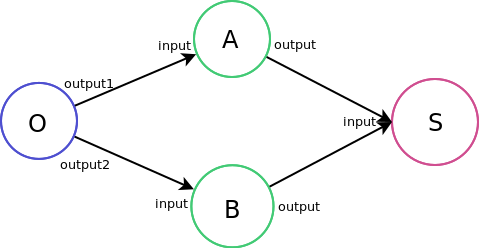
\includegraphics[width=0.8\textwidth]{figures/incdep_lazydep_0}
	\caption{Example figure for illustration in lazy deployment}
	\label{fig:incdep_lazydep_0}
\end{figure}

Apparently \ndS should wait until \ndB propagates the \dEOS marker if \ndB is deployed; \ndS shouldn't wait for the \dEOS marker if \ndB is not deployed. The basic way of tackling this requirement is \ndS checks (\ie probes) whether it is safe to shut down when it receives an \dEOS marker and wait for the reply (\ie answer) to tell it whether it is true or not, which requires a round communication each time \ndS receives a \dEOS (using a counter doesn't help in this scenario because there is no guarantee when the signal to increase the counter will arrive).

There are two options if we don't do probing and answering:
\begin{enumerate}
	\item Increase the to-be-waited number of nodes (by sending signals from the coordinator) for the input connections each time when a new node requires to output through a connection connected to that input connection.
	\item Set the number of nodes to-be-waited to the total possible number of nodes in the beginning.
\end{enumerate}

If we choose method 1, if \ndB delays for a long time and then tries to send data through output connection to \ndS, \ndA will have already finished. In this scenario, the to-be-waited number in \ndS before \ndB requires to send data is \emph{1}, so when \ndA broadcasts \dEOS, \ndS finds the number of total nodes finished has reached \emph{1} so it shuts itself down. A naive, but faulty, patch for this will be set the to-be-waited number larger (e.g. add one) than the actual number, but this will fail when there are more than one nodes requiring to send data at the same time (and finishing sending data before the sink node has received the signals telling it to increase that to-be-waited number. The only way to solve the problem in this method is (with the counter add-by-one in the beginning) to make the coordinator tell the sink that there is another node who will send data to you and wait for \textit{ack} from the sink, which requires round communication between the coordinator and the sink each time for each input connection.

If we choose the second method, when a branch, \eg \ndB, is not (and will never be) deployed because of lazy deployment, the \ndS will never receive the \dEOS from \ndB so the counter will never reach the desired number so the shutdown propagation will fail. The only way to solve this dilemma is to make the coordinator aware when it is the time for \ndS to shut down and tell it to shut down. However, if we choose this approach, it requires more calculations in the coordinator side, which doesn't match our desire to keep the workload of coordinator minimal and will more easily make the coordinator a bottleneck, and there is no need to keep the shutdown propagation because the coordinator now takes control of everything.

What we choose is to also deploy those \tPEInst{}s which are not deployed due to lazy deployment during shutdown propagation. We argue that this method won't create lots of overheads because the coordinator can re-assign these \tPEInst{}s to nodes which has previously shut down. We are aware that there is an extension to this approach which may significantly reduce the number of nodes deployed during the propagation process: do not deploy \tPEInst{}s (and their successors) whose successors (in any depths) will never have input connections connected with the output connections from other parts of the graph. However, because of the time limit, we didn't introduce this to our implementation.

\section{Simple Example} \label{sec:incdep_example}
Here we present a simple solid example to demonstrate how \tincdep works.

Consider a graph doing some simple mathematical calculations like this (illustrated in Figure \ref{fig:incdep_example_0}):
  
\defNodes{A,B,C,D,E}

\begin{itemize}
	\item Two PEs \ndA and \ndB each produces some numbers.
	\item PE \ndC splits the number by their sign: the positive ones go to PE \ndD; the negative ones go to PE \ndE.
	\item PE \ndD sums all positive numbers together.
	\item PE \ndE counts the number of data units it receives.
\end{itemize}

\begin{figure}[h]\centering
    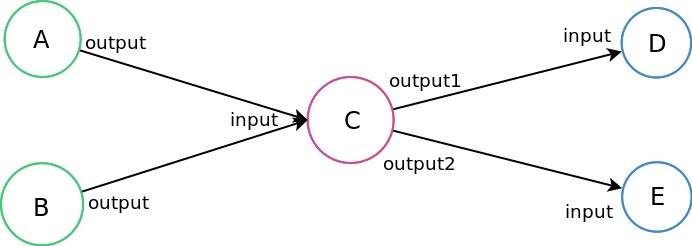
\includegraphics[width=0.8\textwidth]{figures/incdep_example_0}
	\caption{Workflow design}
	\label{fig:incdep_example_0}
\end{figure}

Without \tincdep, \dpy analyses the whole workflow and deploys all nodes at the beginning. But everything goes into incremental steps under \tincdep:

\begin{enumerate}
	\item When initializing, the coordinator is the first initialized and all other nodes are seen as worker nodes which wait for signals from the coordinator by default. The coordinator analyses the workflow, and deploys the first two PEs, \ndA and \ndB.
	\item After deployment, PEs \ndA and \ndB start producing data. Suppose \ndA produces the first unit of data earlier than \ndB. \ndA sends the request with the name of the output, \lstinline|output|, to the coordinator.
	\item The coordinator receives the request, checks and finds \ndC hasn't been deployed. It then deploys \ndC to a free node, say, node 3.
	\item Suppose during this time, the request from \ndB comes to the coordinator. The coordinator knows it is handling the deployment of \ndC, so it simple waits until the completion of the deployment of \ndC.
	\item After deployment, the coordinator sends back the target for the output, \lstinline|output|, of \ndA, and does the same for \ndB.
	\item When A (or B) is producing more data from it output connection \lstinline|output|, it knows it already has the destination, so it won't communicate with the coordinator again.
	\item When \ndC is sending data through output \lstinline|output1| for the first time (suppose \ndC produces data first through \lstinline|output1|), it sends the signal to the coordinator to request the destinations of \lstinline|output1|. Then, \ndD is deployed by the coordinator, and the reply sends back to \ndC.
	\item Similar thing happens for \lstinline|output2| of \ndC.
\end{enumerate}

The steps are illustrated in a series of pictures (see Figure \ref{fig:incdep_example_steps}). After all requests and replies, all nodes are deployed and no duplication will occur. If, for example, output connection \lstinline|output2| of \ndC is never used, \ndE will not be deployed during processing (but, in our implementation, will be deployed when propagating the \dEOS marker as described above).

\begin{figure}[h]\centering
    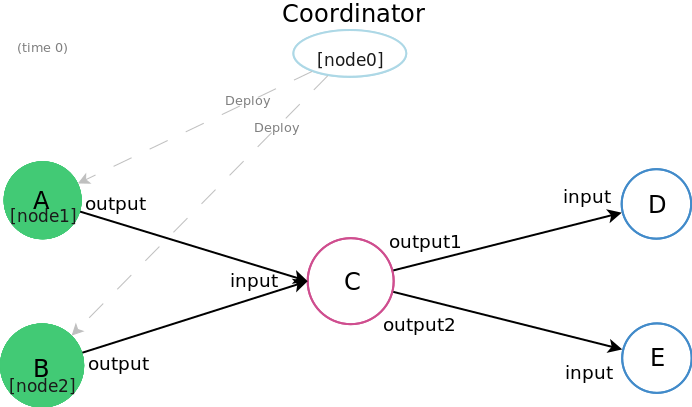
\includegraphics[width=0.4\textwidth]{figures/incdep_example_1}
    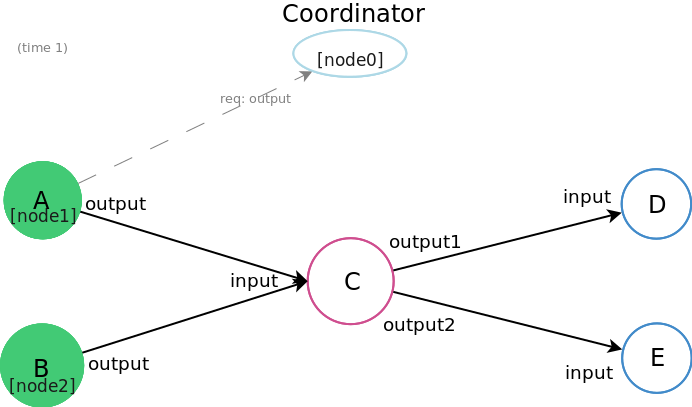
\includegraphics[width=0.4\textwidth]{figures/incdep_example_2}
    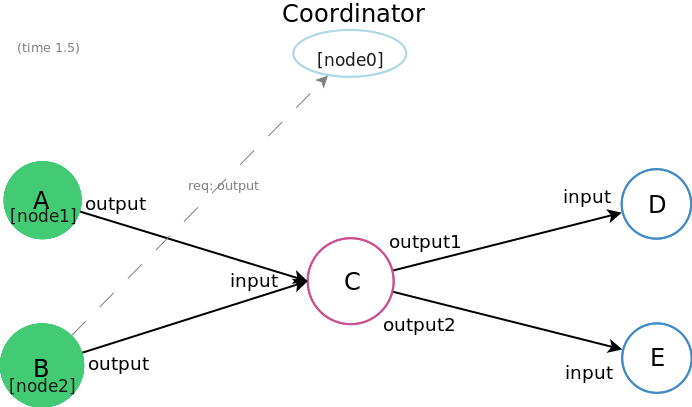
\includegraphics[width=0.4\textwidth]{figures/incdep_example_2_5}
    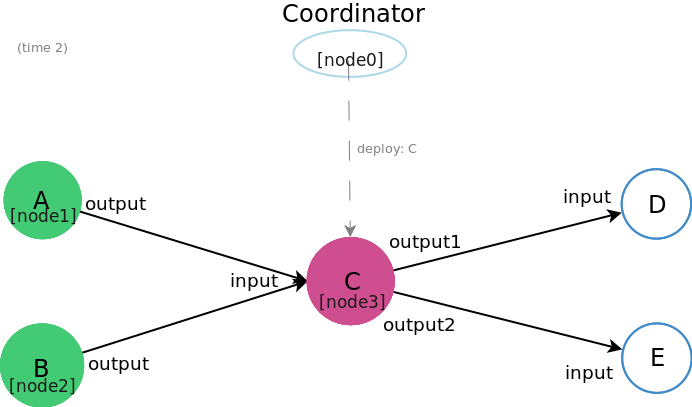
\includegraphics[width=0.4\textwidth]{figures/incdep_example_3}
    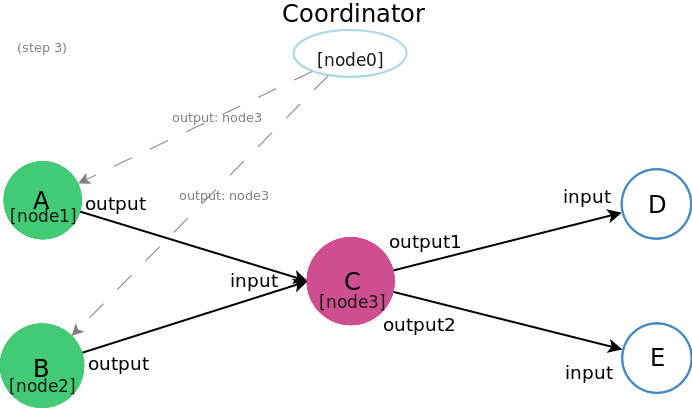
\includegraphics[width=0.4\textwidth]{figures/incdep_example_4}
    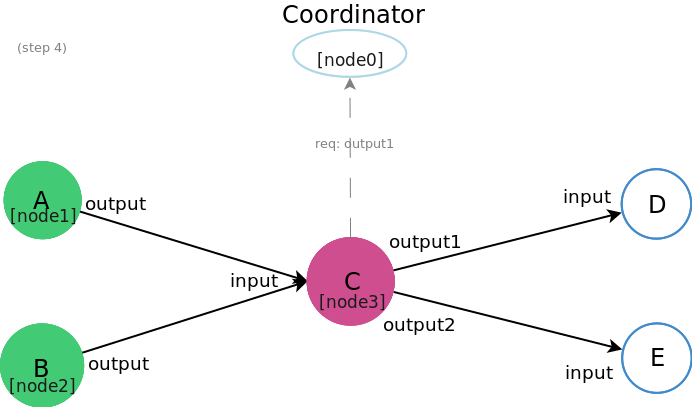
\includegraphics[width=0.4\textwidth]{figures/incdep_example_5}
    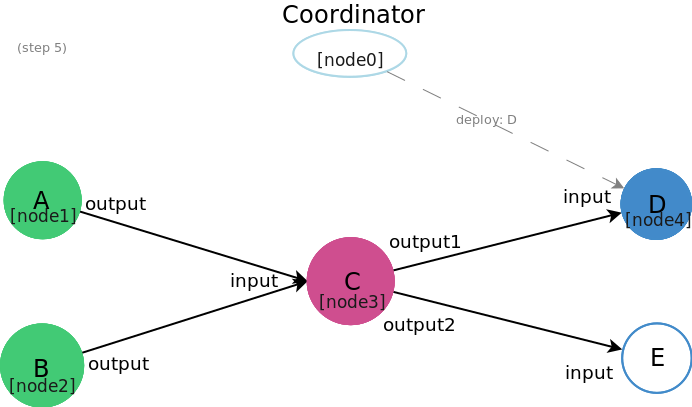
\includegraphics[width=0.4\textwidth]{figures/incdep_example_6}
    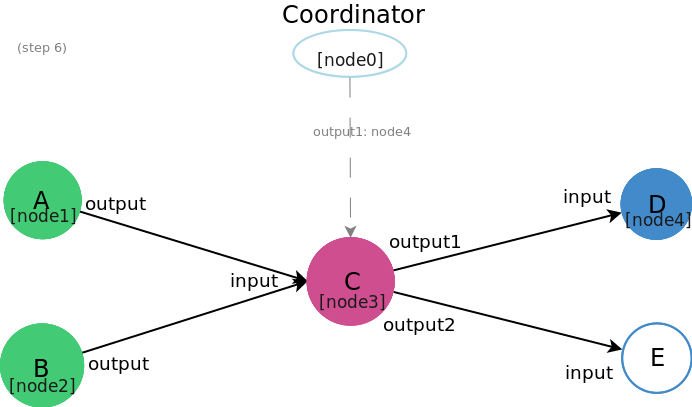
\includegraphics[width=0.4\textwidth]{figures/incdep_example_7}
    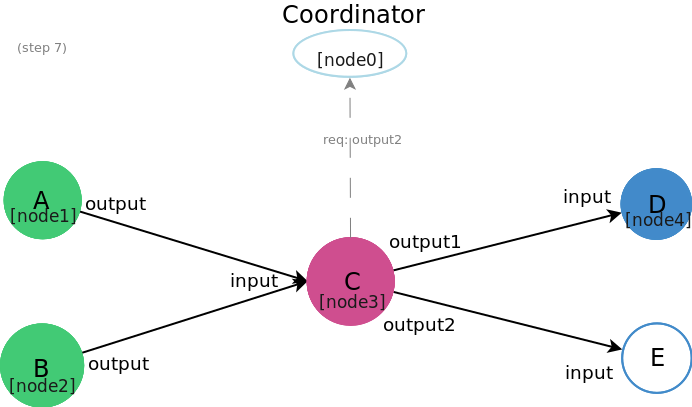
\includegraphics[width=0.4\textwidth]{figures/incdep_example_8}
    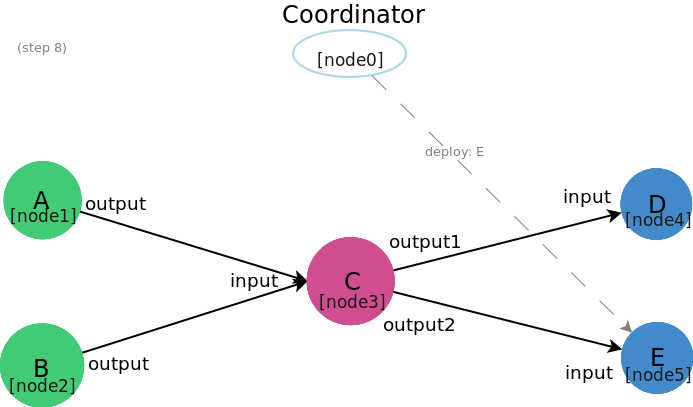
\includegraphics[width=0.4\textwidth]{figures/incdep_example_9}
    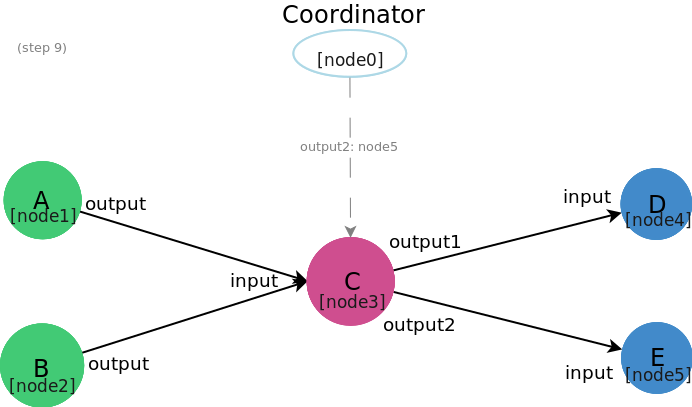
\includegraphics[width=0.4\textwidth]{figures/incdep_example_10}
    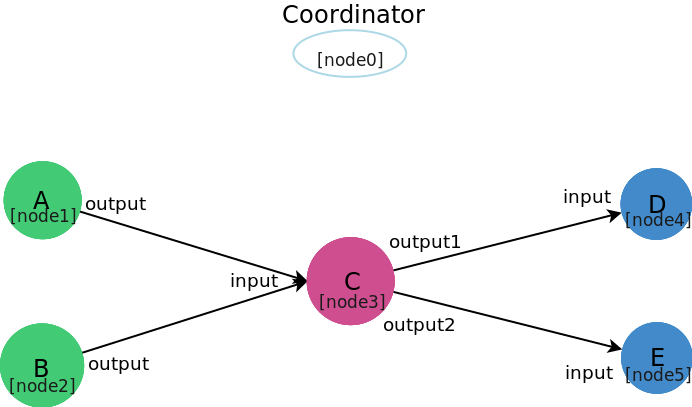
\includegraphics[width=0.4\textwidth]{figures/incdep_example_all}
	\caption{Communication at each time slice}	\label{fig:incdep_example_steps}
\end{figure}

\section{Implementation}
The sections above described the design of the logic, with only a few notes about the implementation. In this section, we describe the issues we encountered during implementation. We first talk about our design of the extension to \dpy, and then present some issues we encountered in each relevant subsection.

Because \tPEInst{}s are unaware of which node its input or output connections are connected to, they can't be executed plainly -- some mechanisms need to handle data transmission. The existing \dpy mechanism uses wrappers on each \tPEInst to handle the input, output and shutdown issues. We kept this design and did some extra work to make the wrapper run correctly under our extension. Details are described in \ref{ssec:incdep_ecs}.

The existing \dpy code supports a mechanism called ``grouping'' so we also need to provide mechanisms to support grouping when implementing our extension in order to keep backward compatibility. To support grouping, we introduce representatives from each group for synchronization (see \ref{ssec:incdep_ecs}).

All these designs are based on ordered messages between each pair of nodes, which is guaranteed by the MPI specification.

\subsection{Efficiency, Concurrency, and Synchronization} \label{ssec:incdep_ecs}
Because all nodes are executed in parallel, the time when a signal or a unit of data will arrive is unpredictable. Therefore, we need to guarantee the correctness under all circumstances. 

For example, when a \tPEInst is going to send a unit of data, it is possible that the reply from the coordinator returns immediately but it is also possible that the reply returns only after a long delay. Usually, handling data transmission is a lot less computational-intensive than processing data. Therefore, it would be more efficient to keep processing more data and leave the waiting and sending in a concurrent thread with suitable buffering.

We use multi-threading to achieve concurrency in the wrapper of \tPEInst, and keep the design of each \tPEInst intact (as there is no guarantee in the specification that calls to the \lstinline|process| method is thread-safe); similarly, the coordinator is also changed to be multi-threaded for better performance.

We can expect many communications to and from the coordinator to run in parallel. Therefore, we will handle each request in a separate thread. Because multiple requests may act on the same PE, we will add a lock to each PE and acquire it when it is going to be acted on (and release it when finished). Thus different requests of this same PE will be sequentialized, so no duplicated deployment will happen.

Because a wrapper reads data from some input connections, processes the data previously read in the \tPEInst it wraps and writes processed output to some output connections, we run ``read'' in one thread, and run ``process'' and ``write'' together in another thread. We are aware that making ``process'' and ``write'' separated and all ``write''s in parallel may very likely achieve better performance, but we didn't implement it because of the time limit. Because we need also request the address of targets (successor nodes), we need to design a suitable place to handle the communication to the coordinator. We decide to send the request when it is needed, and listen in another dedicated thread. The synchronization will be done by using condition variables - wait for the condition variable to become true after sending the request, and set it to true when receiving the reply.

We introduced local leaders (called \emph{representative}s) for each group to keep compatibility of the grouping mechanism. The representative is responsible for synchronization between groups. When a non-representative node wants to terminate its processing because of the shutdown propagation, it waits until all its data has been received and informs its representative that it is going to shutdown. After informing the representative, it informs the coordinator and then shuts down and returns to the listening state. When the representative knows all nodes in its group are going to shutdown, it propagates the \dEOS marker to all proceedings (\ie all input connections receiving streamed data from its group) and shuts itself down (as well as informing the coordinator). It is more natural to let the representative wait for the finish of all data transmissions, but this is not possible in MPI. The only way to ensure all data from a group has been received by the receiver is to use \lstinline|MPI_Issend()| and perform a \lstinline|MPI_Waitall()| to all \lstinline|MPI_Request| objects returned by (every call of) the \lstinline|MPI_Issend()| function. This causes all other nodes (\ie all nodes except for the representative) in the group to wait for longer time before they can inform the representative and actually shut down; on the other hand, this approach does not send information (about how or what to wait for before shutting down) to the representative so the amount of data in the signals is reduced.

\subsection{Spawning}
One of the possibilities \tincdep gives \dpy is it allows \dpy to spawn more nodes when needed (\eg initial nodes are not enough). However, this behaviour also increases the complexity of the code.

Three aspects are affected by supporting spawning:
\begin{enumerate}
	\item Determine and spawn new nodes.
	\item Establish communication between existing and new nodes.
	\item Select the right channel to transmit data / message.
\end{enumerate}

\subsubsection{Determine and Spawn}
Determining when to spawn new nodes is fairly easy: the coordinator simply checks whether there are enough free nodes to be assigned the required \tPEInst{}s. If there aren't enough free nodes, it is very \textbf{likely} the coordinator needs to spawn more nodes. We emphasize the word \textbf{likely} because sometimes there is no need to spawn: for example, when the whole workflow is a line and the data is finite, the head node will finish so the coordinator can wait until it finishes and re-deploy the next \tPEInst to it. However, this behaviour is not steady so we force the coordinator to spawn more nodes once a shortage-of-nodes happens.

We need to ensure all nodes are communicable, so, under MPI specification, all nodes need to collectively spawn the new nodes. This involves a message transmission from the coordinator to make worker nodes aware there is a need to spawn nodes and trigger the spawning function call.

\subsubsection{Establish Communication}
We expect all nodes (at least, all worker nodes) to be able to communicate with each other. We choose to merge the new \emph{Intercommunicator} created by the spawning process into one larger \emph{Intracommunicator}. In this way, we can repeat the same behaviour for spawning more nodes through the newly created \emph{Intracommunicator}.

As discussed previously, we use local leaders (called \textbf{representative}) for each group to suit the existing grouping mechanism which is introduced to increase throughout by (automatically) deploying \tPEDup{}s of the same \tPEInst and processing data in parallel. The communication inside each group is implicated in the way how the synchronization between each group is performed.

As a result, we use three sets of communicators: one for data transmission, one for communication between the coordinator and the worker nodes and one for communication inside each group. We use \lstinline|MPI_Comm_dup()| to achieve this goal, which is a compromise because of the time limit. In principle, these three sets of communications involve different sets of nodes at each deployment so they are not identical to each other; however, in principle, each worker node may communicate with any other worker nodes (both as inter-group and intra-group communications), so does the coordinator. Logically, these three sets of communications can share one promiscuous communicator and we can use different tags or special data fields to distinguish between them. However, the logic is not clear if we don't distinguish these three sets of communications and there is no guarantee about the performance of using the promiscuous communicator.

\subsubsection{Channel Selection}
Because of the introduction of dynamic node spawning and communicator merging, more MPI communicators are created. If an old node needs to communicate with a new node, it must use the newest communicator. However, the order of messages needs to be guaranteed for shutdown propagation, so we can't switch directly from an old communicator to a new one. The situation is even more complicated when we consider the other two sets of communicators.

We use an \emph{existing or newest} concept to select the communicator: if two nodes have already communicated through a communicator, then future communications all go through that communicator; if no communicator has been used between two nodes, then we select the newest one; for communication between worker nodes and coordinator, we keep using the existing communicator during the worker working, and switch to the newest when it's free; for communication inside group, we use the newest communicator when deploying nodes of that group.

	
\chapter{Dynamic Expansion}

	
\chapter{Evaluation and Measurement}
(FIGURE NOT FILLED; NOT YET COMPLETED)

In this chapter, we show that our modification to \dpy keeps backward compatibility and extends the semantics. We also show the performance of our modification on several tasks and platforms.

To show the performance, we need first describe what platforms and what workflows we choose to perform the measurement.

\section{Incremental deployment}
\sout{How to measure, what to measure  (mainly those described in the measurement plan).
Results (figures) and analysis.}

\section{Dynamic expansion}
Dynamic expansion is the new property we have added to dispel4py system. It creates a new semantics to workflow design so that workflows can grow / expand according to needs. We use the sieve of Eratosthenes to demonstrate the potential usage of this new semantics, and make comparisons between the approaches we need to construct such a workflow graph in both the old system and our new system, and the performance of the old system (constructed in the old way) and the new system (constructed in the new way).

The idea of \tsieve was described in the Use Cases chapter. To write a workflow which utilizes the sieve of Eratosthenes without \emph{dynamic expansion},  researchers need to first write down the range of numbers (which is always needed), and then estimate (or calculate) the number of primes inside this range. This is a chicken-and-egg problem: we need to execute the whole workflow to know \textbf{what} primes are there inside this range and then can know the \textbf{number} of primes inside this range; but we also need the \textbf{number} of primes to design the workflow (which is prior to the execution of this workflow). Therefore, there are two ways to ``solve'' this problem:
\begin{enumerate}
	\item Run the calculation somewhere else and use that result.
	\item Estimate a bigger number and hope the actual number of primes won't exceed it.
\end{enumerate}

Apparently these two ways are not neat, and there isn't a neat way to solve this problem in the old semantics. However, in our new system with \emph{dynamic expansion}, this problem automatically goes away: researchers simply need to define when to dynamically expand this node as a part of the construction of the Sieve PE, and add \textbf{one} of it into the workflow. Figure \ref{fig:comp_old_new_sieve} shows the structure of workflow design in the old system and the new system.

\begin{figure}[h]
\caption{
TWO FIGURES HERE:
the first one shows the structure of the old semantics (with one IntegerProducer and many Sieves);
	the second one shows the structure of the new semantics (with only two nodes: IntegerProducer and Sieve)
}
	\label{fig:comp_old_new_sieve}
\end{figure}

The results are shown in Figure \ref{fig:sieve_all_100} and \ref{fig:sieve_all_1000}; Figure \ref{fig:sieve_opt_100} and \ref{fig:sieve_opt_1000} only compare the static constructed workflow run in the original MPI mapping with the optimized version of \tdynexp. In all figures, the second column of the legend indicates the platform and the version (separated by a dash), and the third column of the legend is one of the parameters controlling the number of nodes spawned at the beginning.

\begin{figure}[h]
\centering
    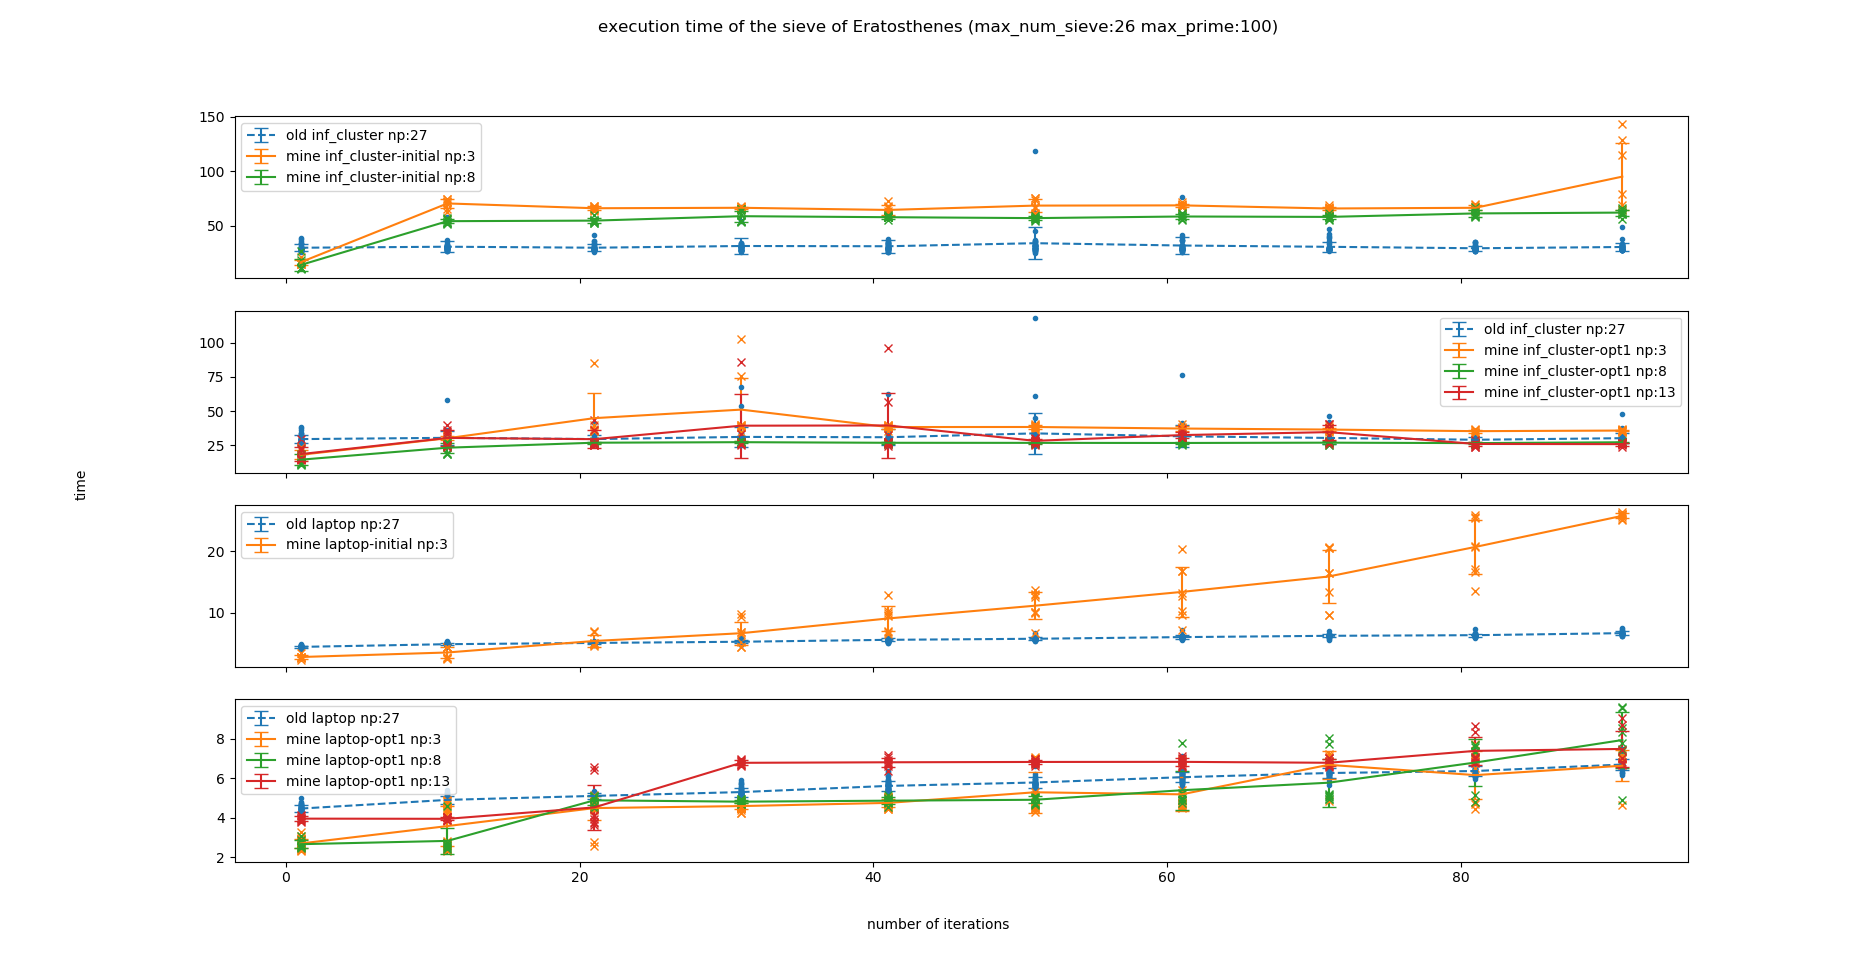
\includegraphics[width=1\textwidth]{figures/sieve_all_100}
\caption{Execution time of the prime sieve to find prime up to 100 on both the old semantics and our new semantics}
\label{fig:sieve_all_100}
\end{figure}

\begin{figure}[h]
\centering
    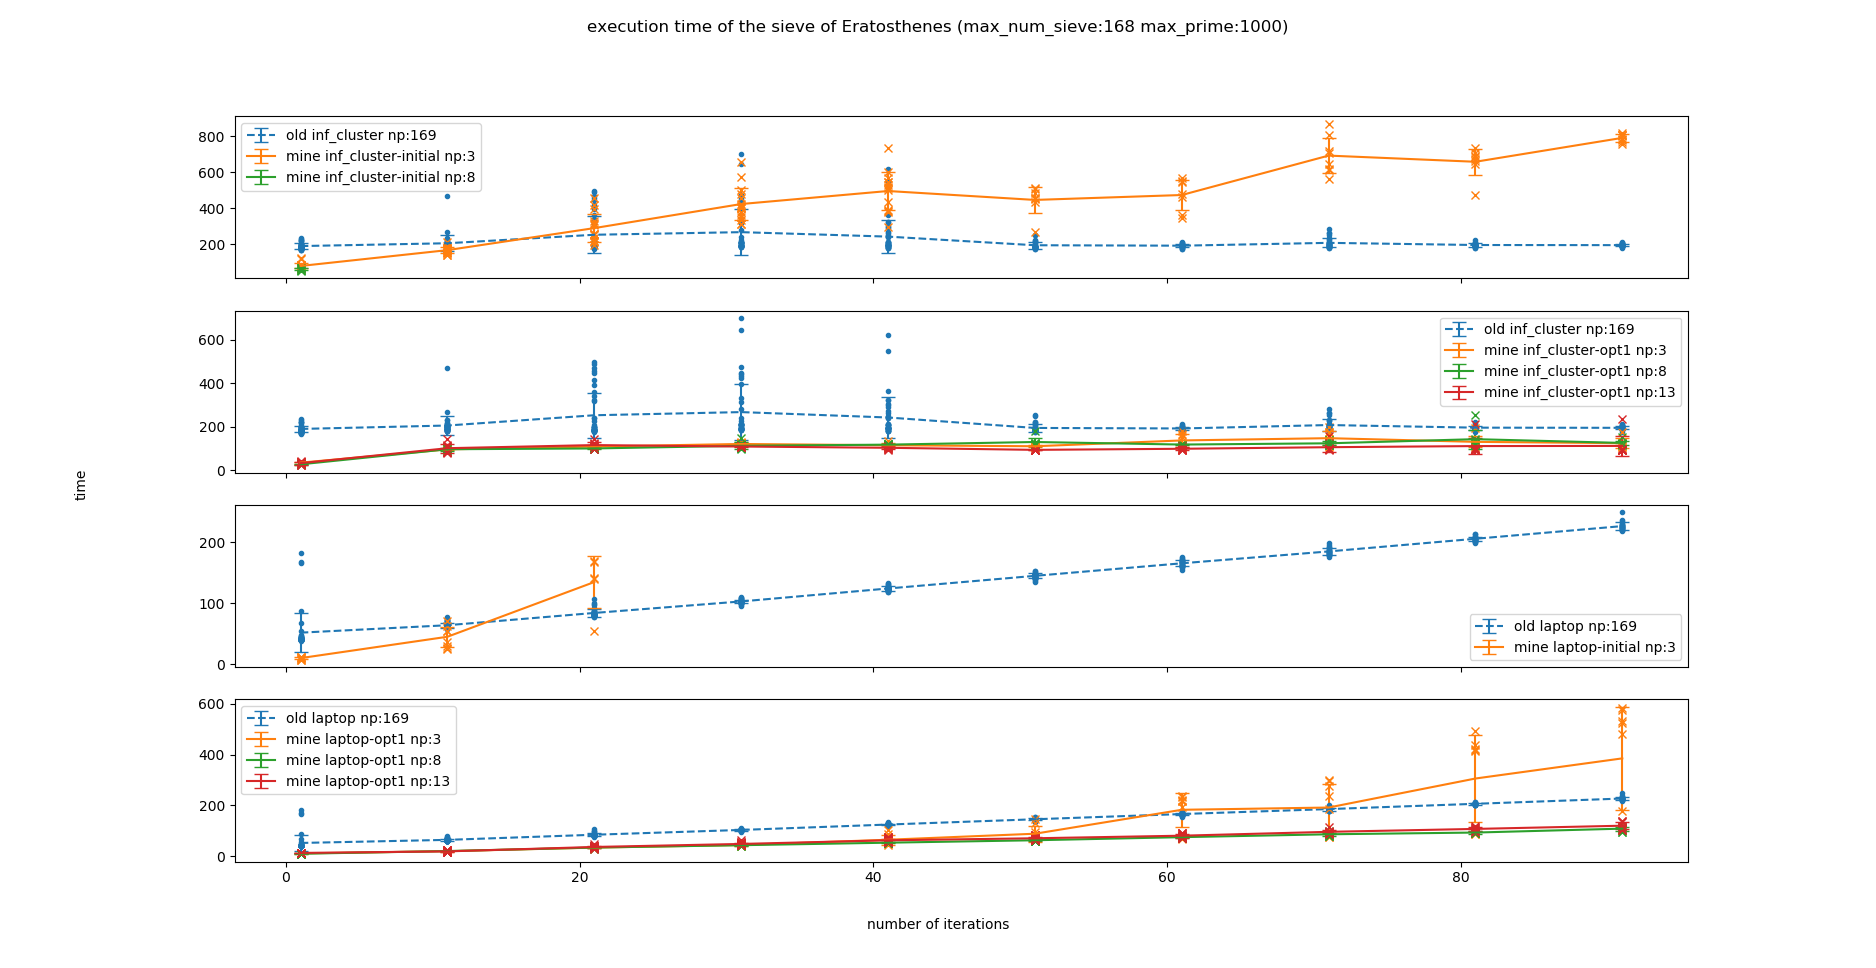
\includegraphics[width=1\textwidth]{figures/sieve_all_1000}
\caption{Execution time of the prime sieve to find prime up to 1000 on both the old semantics and our new semantics}
\label{fig:sieve_all_1000}
\end{figure}

\begin{figure}[h]
\centering
    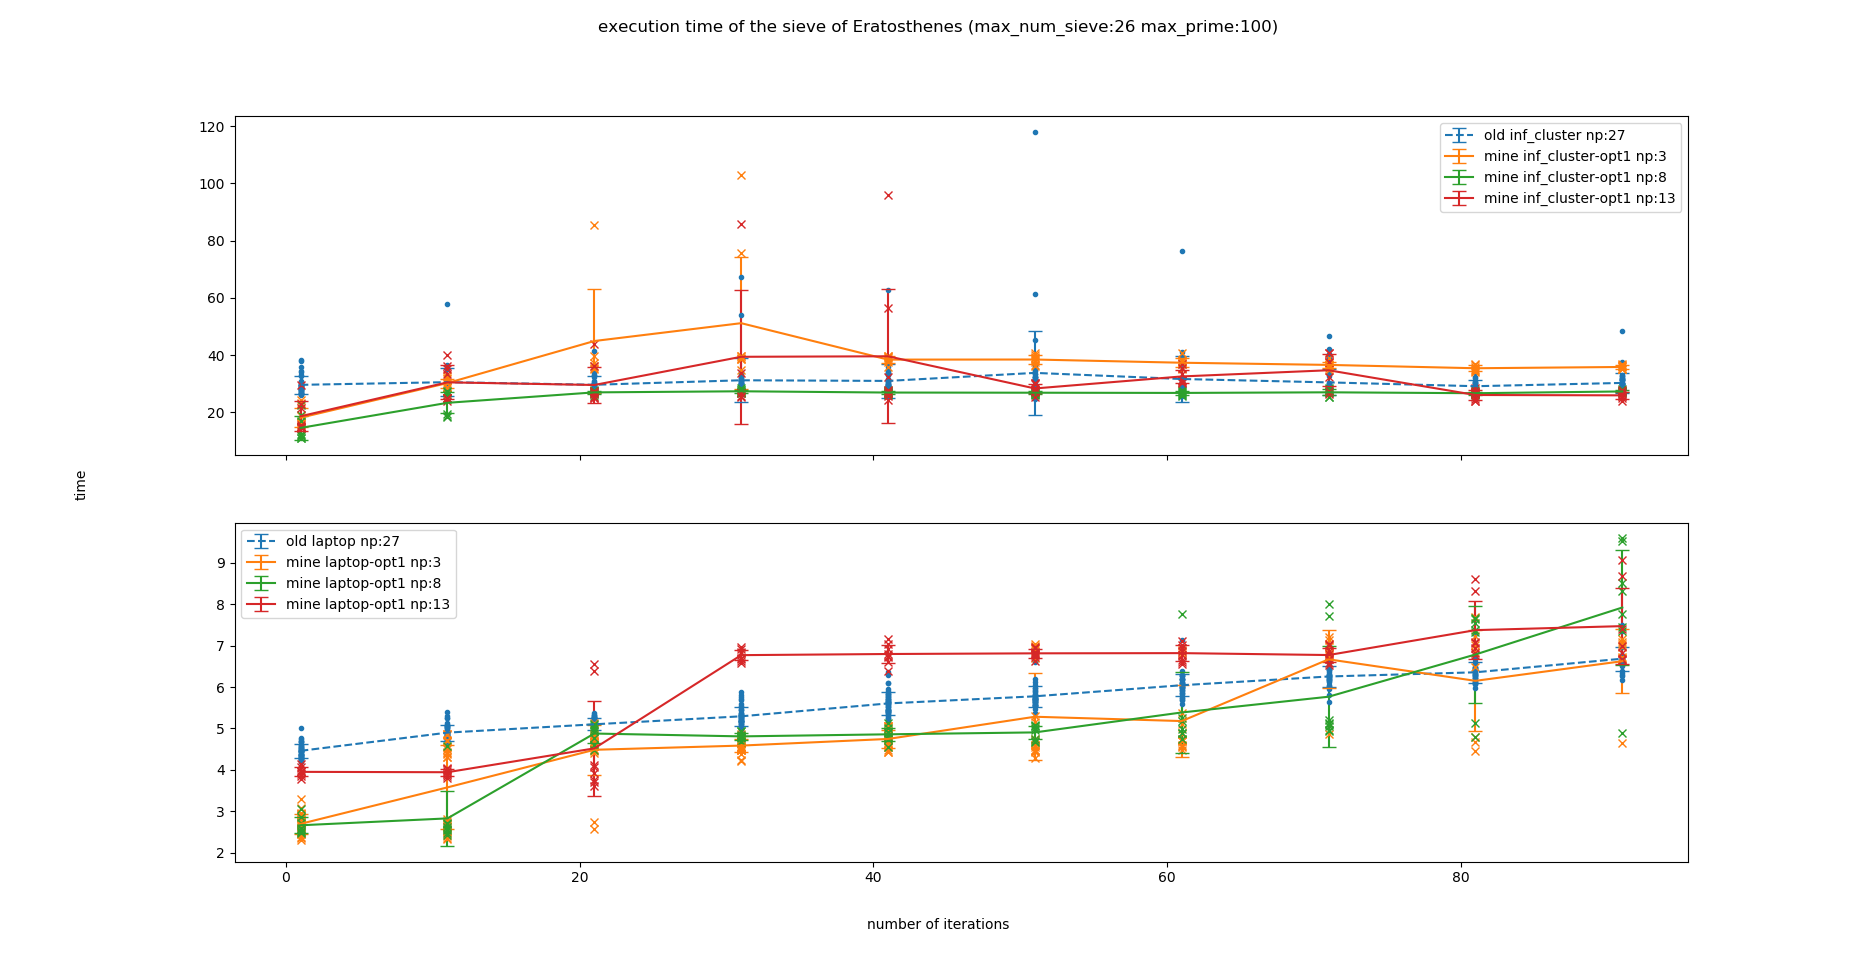
\includegraphics[width=1\textwidth]{figures/sieve_opt1_100}
\caption{Execution time of the prime sieve to find prime up to 100 on both the old semantics and our new semantics (only the optimized version)}
\label{fig:sieve_opt_100}
\end{figure}

\begin{figure}[h]
\centering
    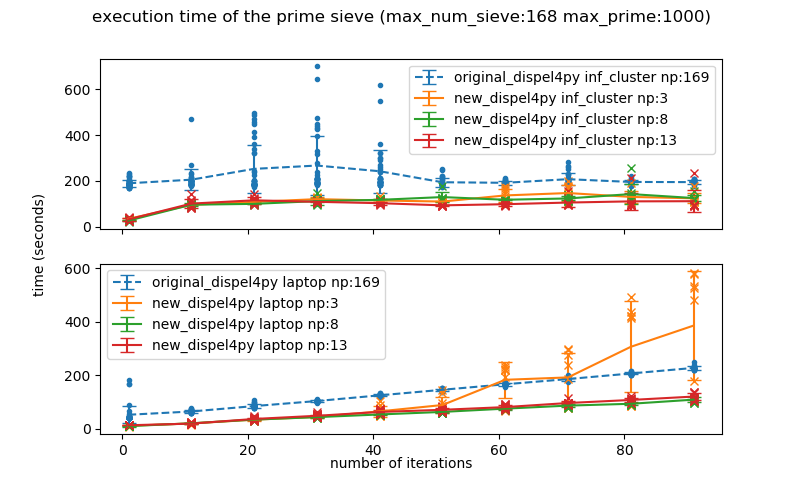
\includegraphics[width=1\textwidth]{figures/sieve_opt1_1000}
\caption{Execution time of the prime sieve to find prime up to 1000 on both the old semantics and our new semantics (only the optimized version)}
\label{fig:sieve_opt_1000}
\end{figure}


\chapter{Conclusion and Future Work}
In this document, we presented the important role of scientific workflows for today's scientific research, the classification of workflow management systems (WMSs) and \dpy, a data-streaming WMS. They formed the the background to our work. Then, we discussed two extensions, \tincdep and \tdynexp, to (the MPI mapping of) \dpy, both give \dpy more dynamics and enable further extensions or optimization. We described our design and implementation which are on the system side of \dpy so they are transparent to researchers / designers of workflows. Finally, we presented our evaluation and measurement of our extension and showed that our extension gives \dpy more dynamics at a low cost and sometimes even with better performance.

Our extensions to \dpy, \tincdep and \tdynexp, jointly form a significant starting point for future extensions or optimizations to \dpy or other data-streaming WMSs. For example, one can utilize and extend \tincdep to dynamically schedule PEs to the most appropriate nodes, or utilize and extend the \tdynexp mechanism to enable more complex runtime workflow self-management behaviours\footnote{Some options are described in the \rcpt{Future Work} section below.}.

The time limit prevented us from exploring measurement with representative sets of workflows. We are also aware of the limitation in our implementation. For example, the single coordinator may become a bottleneck if communication increases; frequent manipulations on MPI communicators may also affect the performance. Possible extensions or optimizations are described in the rest of this chapter, so we or other developers can extend our work. Even though, we consider we have made good progress during the MSc dissertation period.

\section{Future Work}
The rest of this chapter will describe possible future work. They consist of two aspects:
\begin{enumerate}
	\item Potential optimizations to our current implementation;
	\item Possible extensions built upon our work.
\end{enumerate}

If we were allowed more time, we would explore the potential optimizations first, and then the extensions.

\subsection{Potential Optimizations}
In our current implementation, there are some compromises (which have been briefly mentioned in the preceeding chapters) because of the time limit. Given enough time, we would explore which ways will be better. These optimizations are considered by us:

\begin{enumerate}
	\item The \emph{process} and \emph{write} steps are combined together, and they are concurrent with the \emph{read} steps during processing. However, all three can be executed in parallel in principle. Other aspects, such as listening to signals from the coordinator and performing actions, can also be executed in parallel in principle.
	\item When spawning more nodes, the current implementation always spawns a fixed pre-defined number of nodes. However, there may be a smart way to specify this number dynamically according to the workloads and known application behaviour.
	\item After spawning new nodes, the current implementation will connect all nodes together (by merging the \emph{intercommunicator}) in one \emph{intracommunicator} in order to make all worker nodes inter-communicable. However, in the MPI implementation, the merging operation takes time and during this time no data / message can be transmitted. We will call \lstinline|Comm.Dup()| to the merged \emph{intracommunicator}, which makes the time consumption even larger. We expect a better method to handle this process so working nodes don't have to wait.
	\item When establishing communication between nodes, the current implementation uses an \emph{existing or newest} strategy (described in the \tIncDep chapter) to select MPI \emph{communicator}s. This behaviour is introduced because of dynamic spawning and is subject to change if point 3 is changed.
\end{enumerate}

\subsection{Possible Extension}
We consider our work an important step towards further extension or optimization of \dpy. Here, we present some possible further extensions or optimizations based on our extension. \\

\textbf{Extending to other mappings of \dpy}\quad
As we said in the prior part of this document, \dpy can map the same workflow to many execution platforms / frameworks. This indicates that the workflow design in \dpy is platform-neutral. However, our implementation only builds on top of one of the mappings, MPI, because of the time limit. In principle, these extensions can also be adopted to other mappings and become a feature of the whole \dpy system. \\

\textbf{Dynamic scheduling}\quad
When executing workflows, it is always better to deploy PEs smartly to reduce the time consumed for data transmission or to deploy more computation-intensive PEs to powerful nodes and less computation-intensive PEs to less powerful nodes. Therefore, it is useful to be able to deploy PEs to specific nodes according to certain factors (\eg performance data), but this is an NP-hard problem. There are some work (\eg \cite{teylo2017hybrid}) focusing on static scheduling which use prior knowledge or performance data from previous runs; however, building upon our work, future development can gather not only this kind of data but also data from the current run. Moreover, if the deployment of \tPEInst{}s can be moved from one node to another, the runtime performance data will be more useful. \\

\textbf{Auto bundling}\quad
The workload of different PEs are not balanced in nature, meaning some PEs may have heavy computational jobs while some others may have very light ones. By bundling some light PEs together, the network traffic will become local data transmission so throughput will increase because local data transmission / sharing is significantly faster than network traffic. Moreover, less nodes are required so we may be able to utilize these free nodes to run more computation-intensive PEs (or \tPEDup{}s) to achieve better performance. \\

\textbf{Regionalized coordinator}\quad
We use a single coordinator in our implementation, which may consequently become a bottleneck (either to communication or computation). Some properties of the specific workflow graph may be useful to ease this constraint: we may analyse the workflow graph and identify separate regions (\eg connected by one PE) and assign each region one coordinator so each coordinator is only responsible for its region. This may be especially useful when the communication between worker nodes and the coordinator is expensive. \\

\textbf{Pre-deployment}\quad
It takes time from identifying the needs to deploy a PE to be aware the PE has been deployed. It may be better to deploy PEs previous to a corresponding request. However, whether this will contribute to reducing the total time or not is unknown before actually implementing it, and it is also unknown, though with some heuristics (\eg one step prior), how to identify which PEs to deploy. \\

\textbf{Dynamic construction}\quad
In the current \dpy semantics, PEs are constructed before the execution of the workflow. It violates the semantics if the system modifies the PEs outside of them, and forces us to design \tincdep and \tdynexp as they are now for backward-compatibility. However, if we can construct PEs or at least modify some of its properties (in an approved explicit way) during runtime, we can make the dynamics of \tdynexp more robust -- by changing the parameters used to construct the divisional PE to change its behaviour (from the coordinator side), rather than by message passing between PEs. This behaviour may be especially useful if we want to apply the existing grouping mechanism to expandable PEs. Specially, if we can construct PEs during runtime, \tincdep could scale better because worker nodes can construct PEs without knowing the actual workflow. 


%%%%%%%%
%% Any appendices should go here. The appendix files should look just like the
%% chapter files.
%\appendix
%\include{appendix1}
%% ... etc...

%% Choose your favourite bibliography style here.
%\bibliographystyle{apalike}
\bibliographystyle{plain}

%% If you want the bibliography single-spaced (which is allowed), uncomment
%% the next line.
% \singlespace

%% Specify the bibliography file. Default is thesis.bib.
\bibliography{dissertation_bib,sieve}

%% ... that's all, folks!
\end{document}
